\documentclass[a4paper,14pt]{extarticle}

\usepackage[a4paper,top=20mm,bottom=20mm,left=30mm,right=10mm]{geometry}
\usepackage[T1,T2A]{fontenc}
\usepackage[utf8]{inputenc}
\usepackage[russian]{babel}
\usepackage{indentfirst}
\usepackage{titlesec}
\usepackage{graphicx}
\usepackage{verbatim}
\usepackage{fancyvrb}

\renewcommand{\baselinestretch}{1.3}
\setlength{\parindent}{12.5mm}
\titleformat{\section}{\normalsize\bfseries}{\indent\thesection}{1em}{}
\titleformat{\subsection}{\normalsize\bfseries}{\indent\thesubsection}{1em}{}

\begin{document}

  \newpage\thispagestyle{empty}
  \begin{center}
    \MakeUppercase{
      Министерство науки и высшего образования Российской Федерации\\
      Федеральное государственное бюджетное образовательное учреждение высшего образования\\
      <<Вятский Государственный Университет>>\\
    }
    Институт математики и информационных систем\\
    Факультет автоматики и вычислительной техники\\
    Кафедра электронных вычислительных машин
  \end{center}
  \vfill

  \begin{center}
    \textbf{Связность графов}\\
    Отчёт по лабораторной работе №5\\
    по дисциплине\\
    <<Дискретная математика>>\\
    Вариант 8
  \end{center}
  \vfill

  \noindent
  \begin{tabular}{ll}
    Выполнил студент гр. ИВТб-1301-05-00 \hspace{5mm} &
    \rule[-1mm]{25mm}{0.10mm}\,/Макаров С.А./\\
    
    Руководитель преподаватель & \rule[-1mm]{25mm}{0.10mm}\,/Пахарева И.В./\\
  \end{tabular}

  \vfill
  \begin{center}
    Киров 2025
  \end{center}

  \newpage
  \section*{\hspace{12.5mm}Цель}
  Цель лабораторной работы: изучение основ теории графов, формирование матрицы связности, разработка приложения на языке Паскаль или СИ согласно заданию.

  \section*{\hspace{12.5mm}Задание}
  Граф задан матрицей инцидентности в файле (вершин >= 4, дуг >= 4). Сформировать матрицу связности. Определить является ли граф несвязным.

  \section*{\hspace{12.5mm}Решение}

  Для решения задач подготовлен ориентированный граф, представленный на рисунке 1.

  \begin{figure}[h]
    \centering
    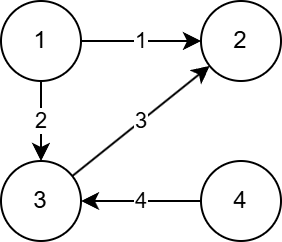
\includegraphics[width=0.4\linewidth]{images/graph.png}
  \end{figure}
  \begin{center}
    Рисунок 1 – Ориентированный граф
  \end{center}

  \pagebreak
  Перед разработкой составлены схемы алгоритмов для решения задач. На рисунке 2 представлены схемы подпрограмм ввода и вывода матрицы.

  \begin{figure}[h]
    \centering
    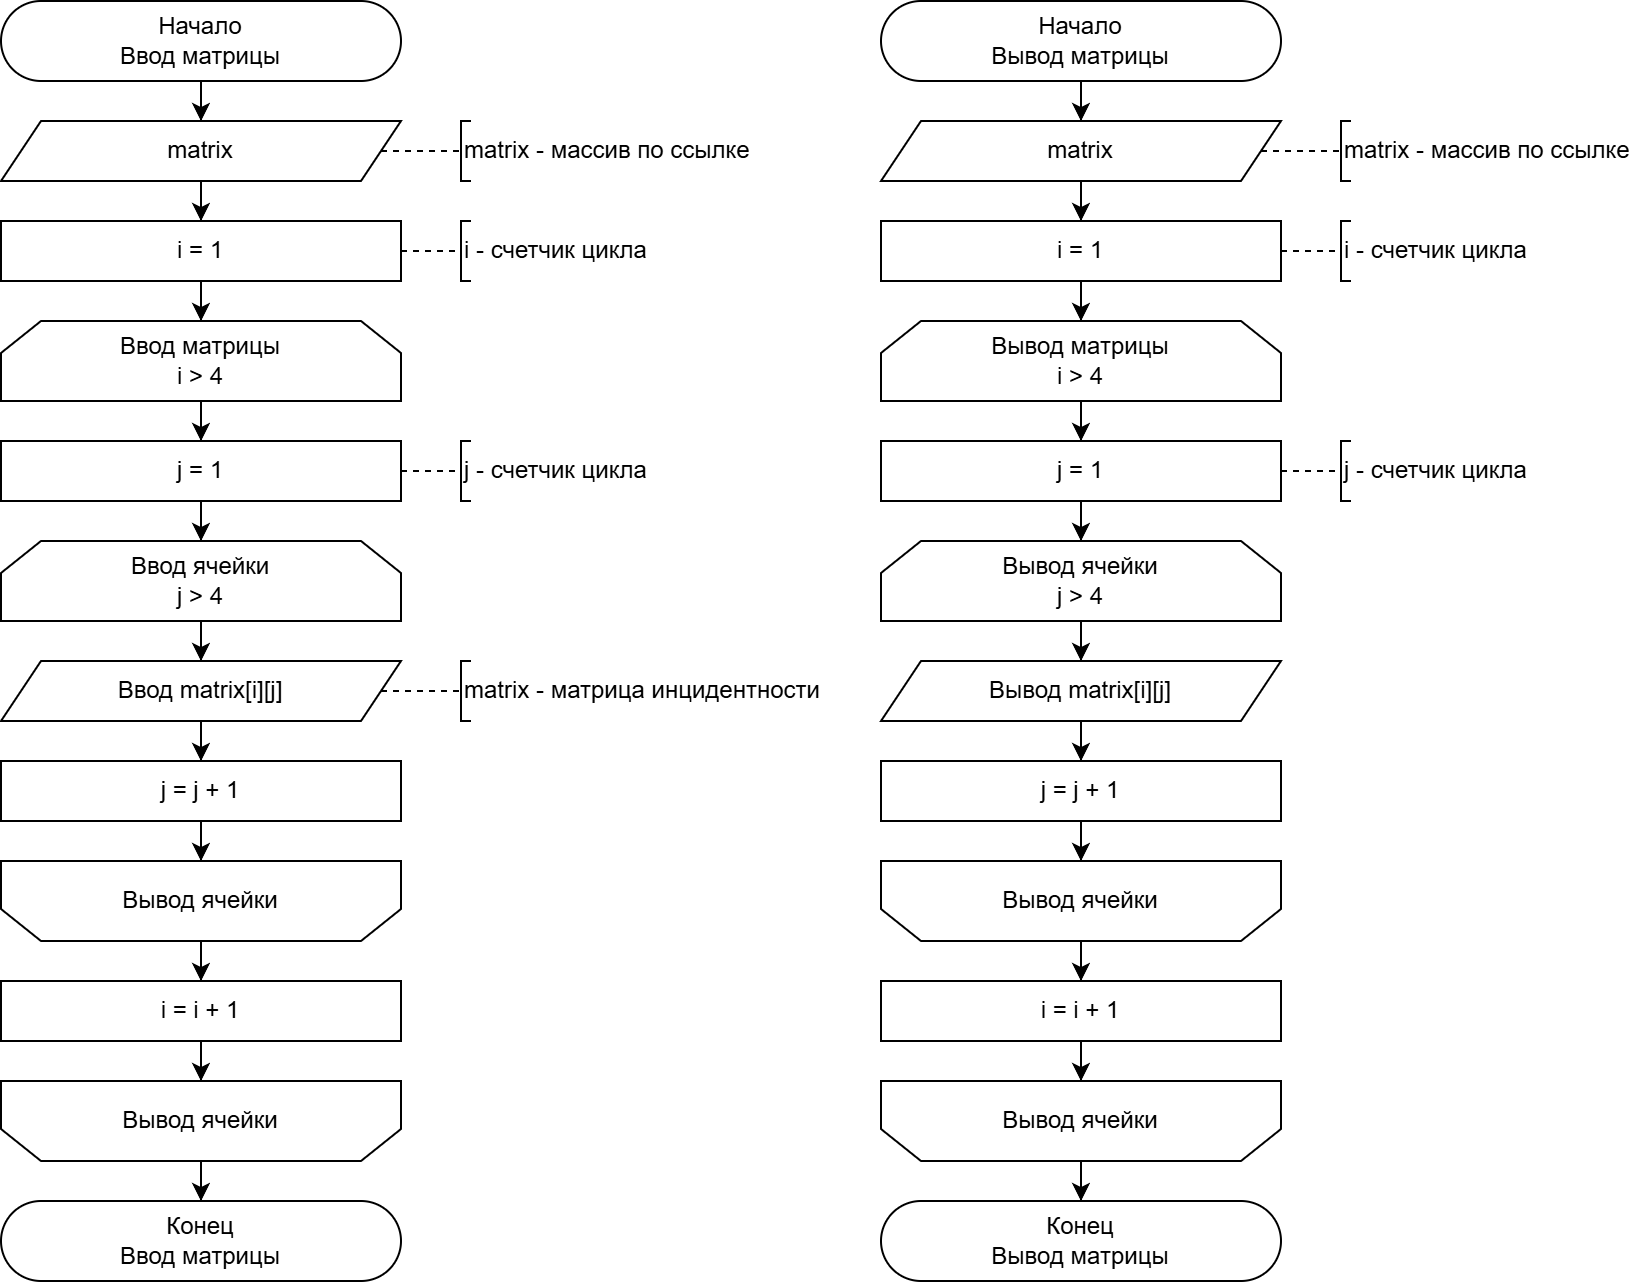
\includegraphics[width=1\linewidth]{images/s-1.png}
  \end{figure}
  \begin{center}
    Рисунок 2 – Схемы алгоритмов ввода и вывода матрицы
  \end{center}

  \pagebreak
  На рисунке 3 представлена схема подпрограммы перевода матрицы инцидентности в матрицу смежности.

  \begin{figure}[h]
    \centering
    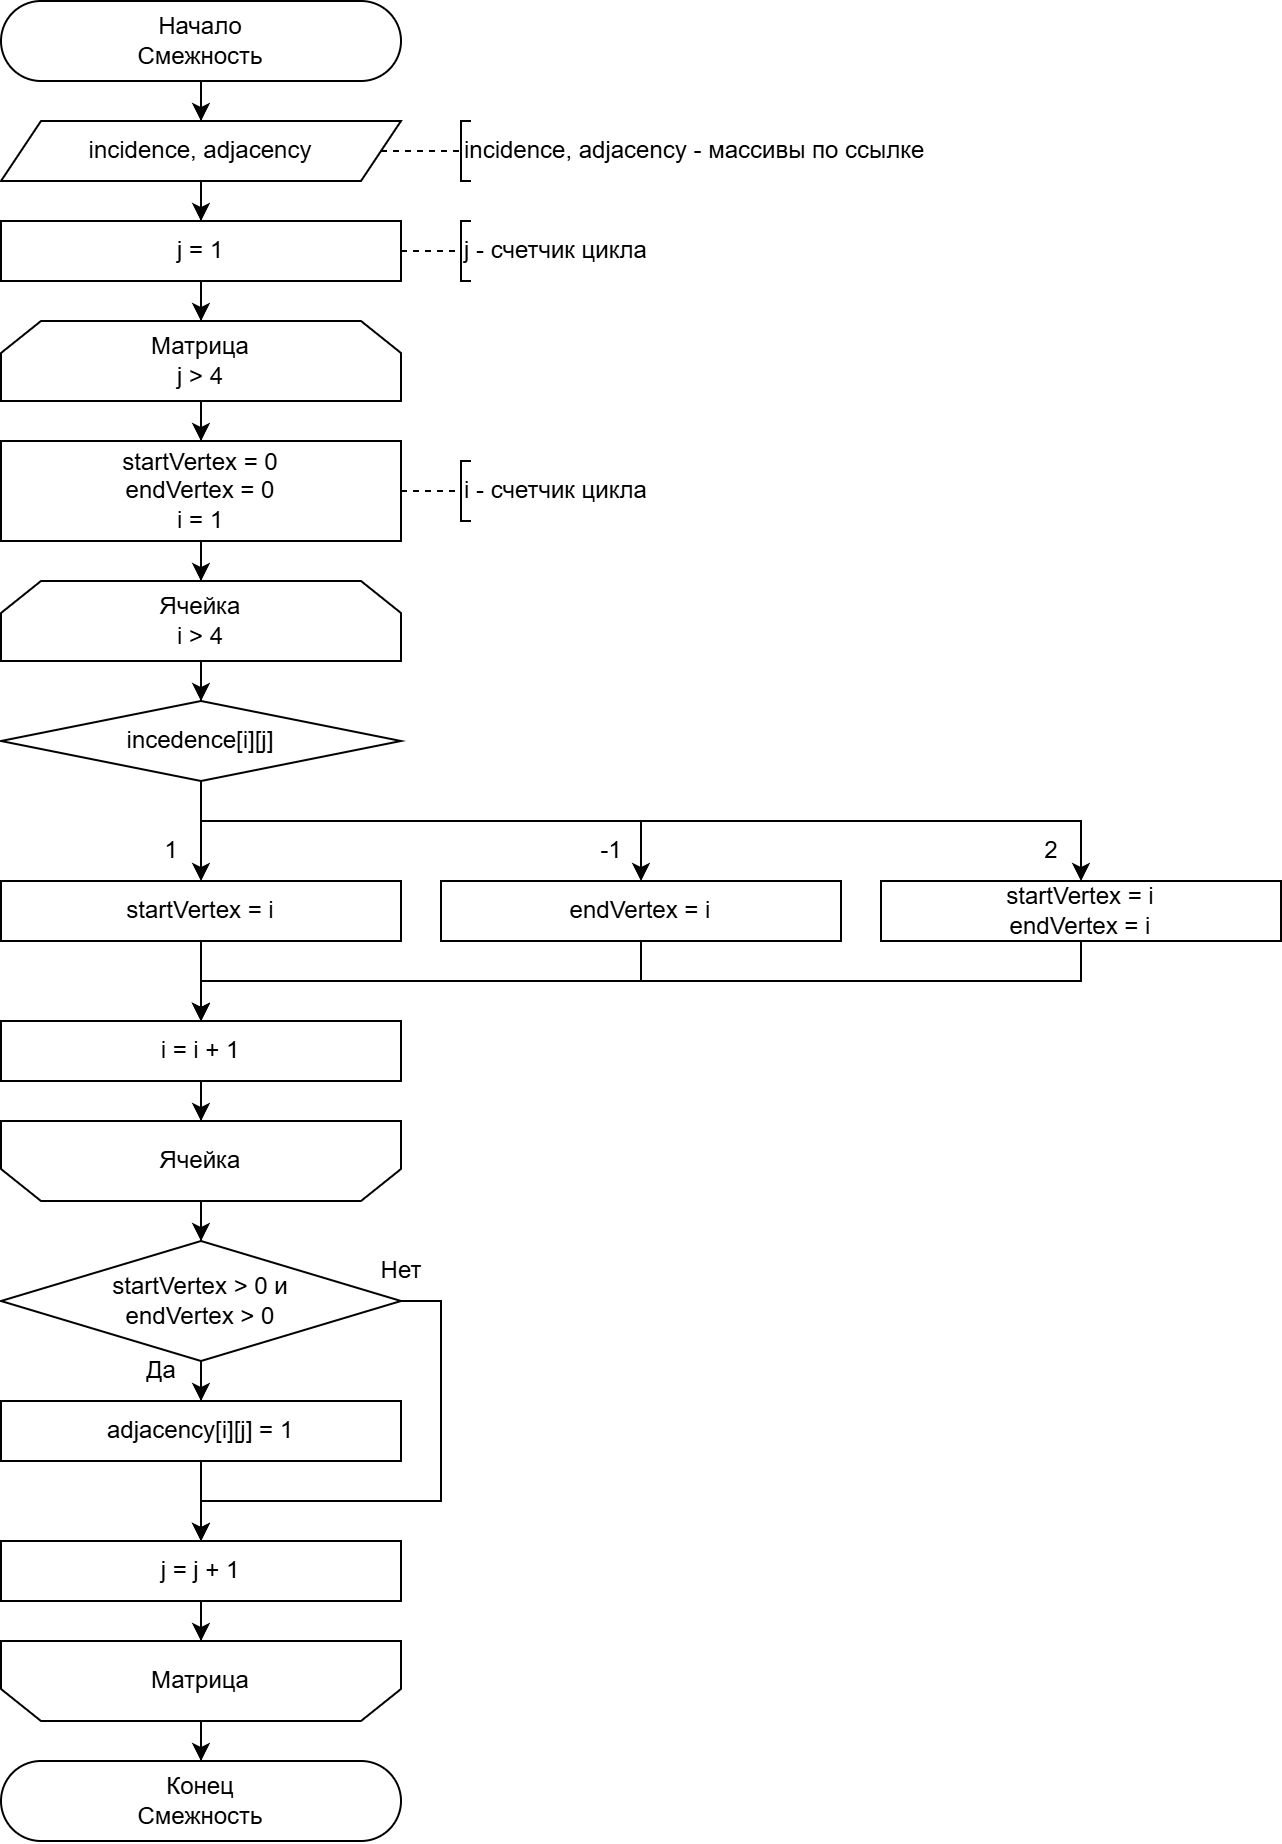
\includegraphics[width=0.8\linewidth]{images/s-2.png}
  \end{figure}
  \begin{center}
    Рисунок 3 – Схема алгоритма перевода в матрицу смежности
  \end{center}

  \pagebreak
  На рисунке 4 представлены схемы подпрограмм умножения и сложения матриц.

  \begin{figure}[h]
    \centering
    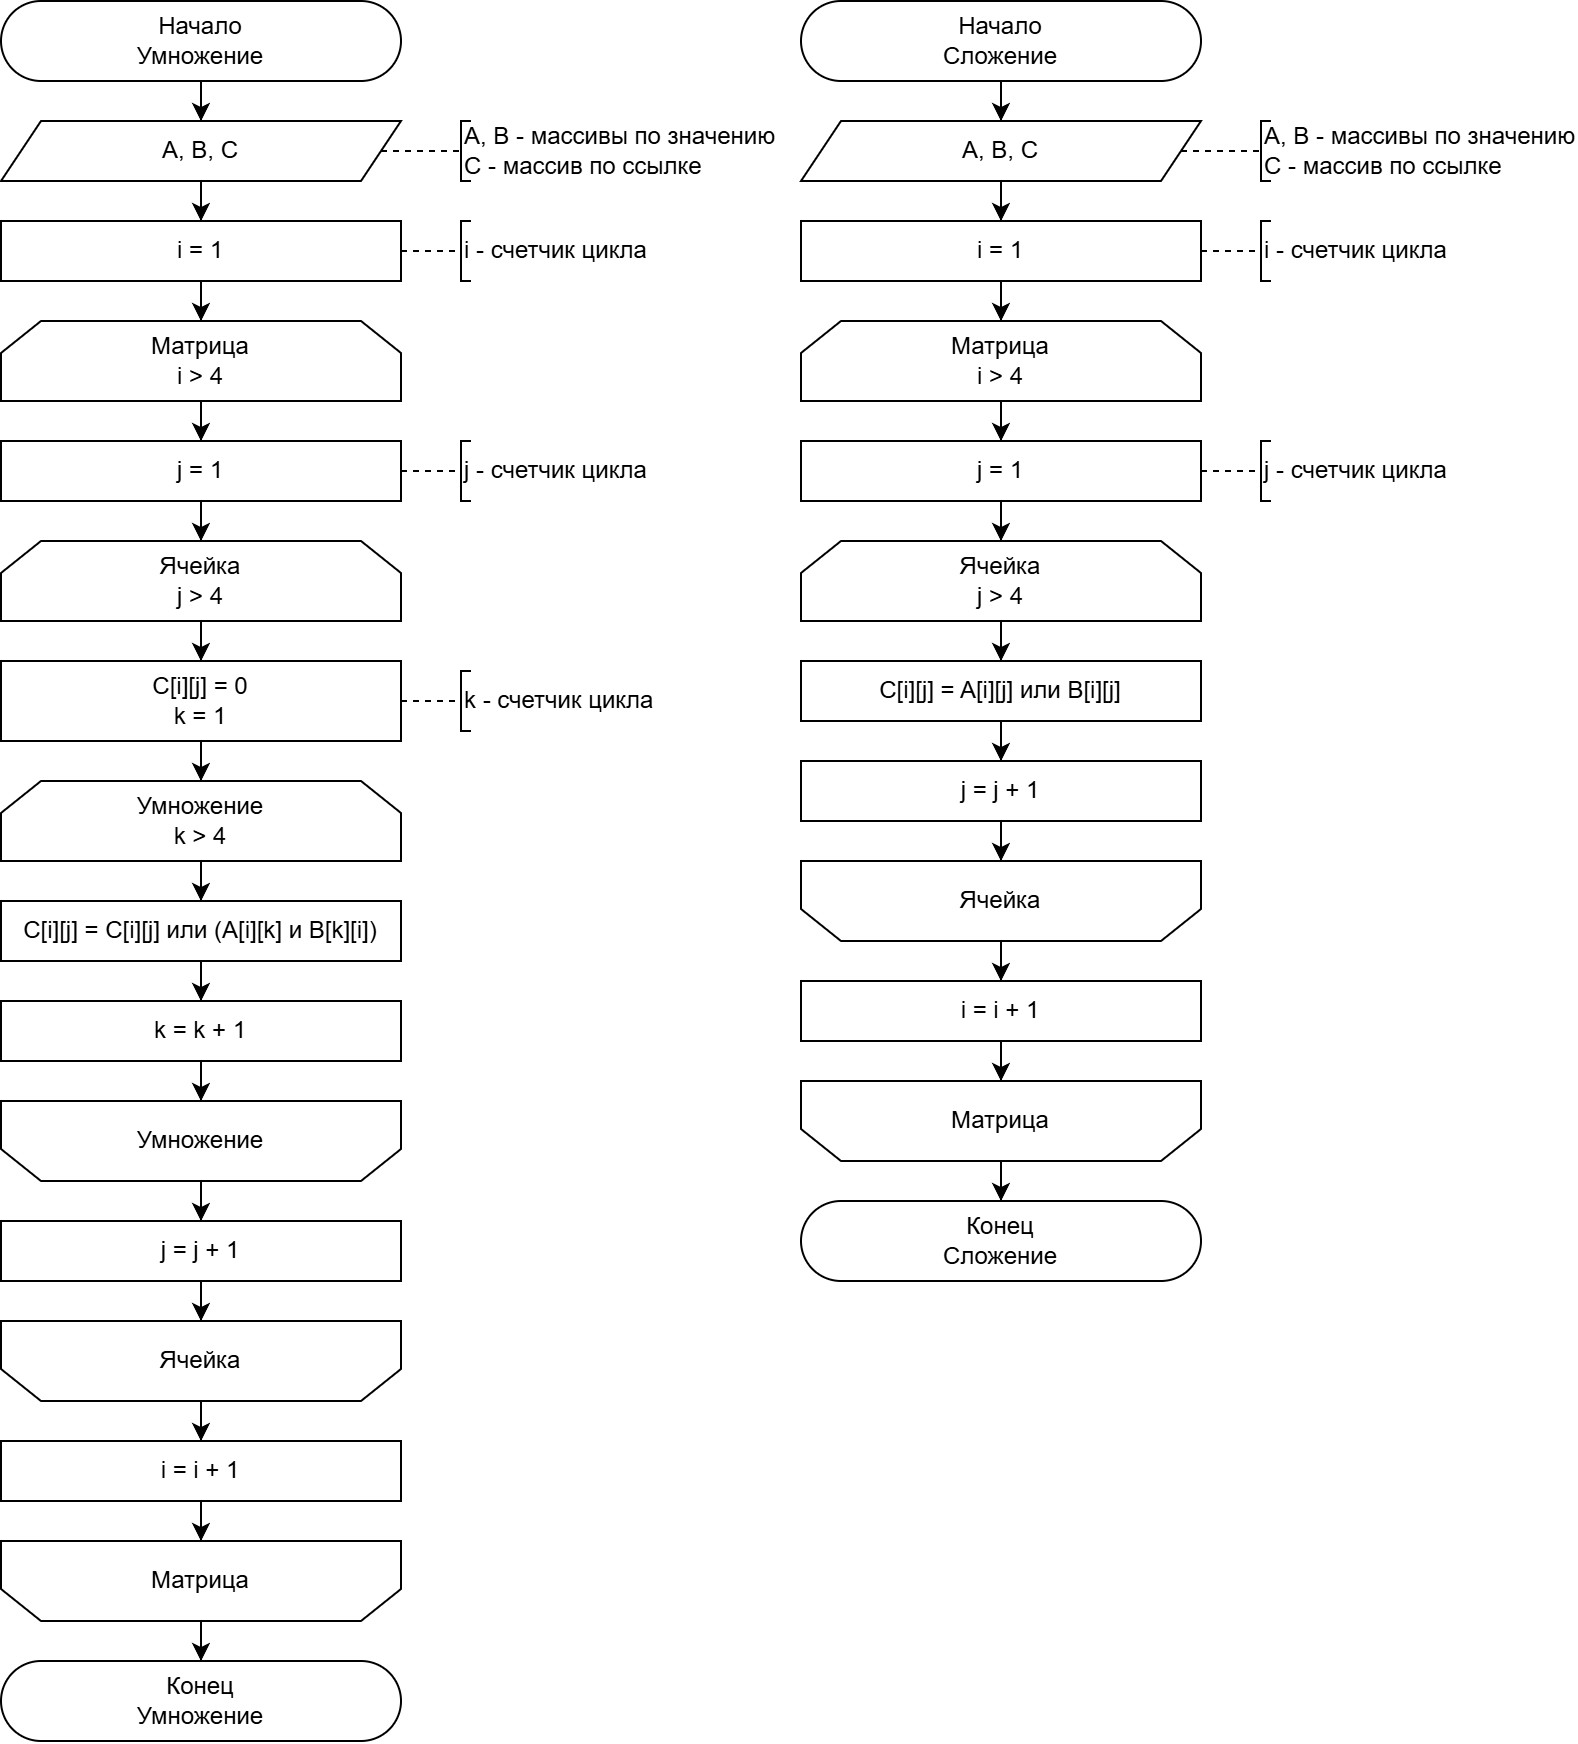
\includegraphics[width=1\linewidth]{images/s-3.png}
  \end{figure}
  \begin{center}
    Рисунок 4 – Схемы алгоритмов умножения и сложения матриц
  \end{center}

  \pagebreak
  На рисунке 5 представлена схема подпрограммы формирования матрицы достижимости.

  \begin{figure}[h]
    \centering
    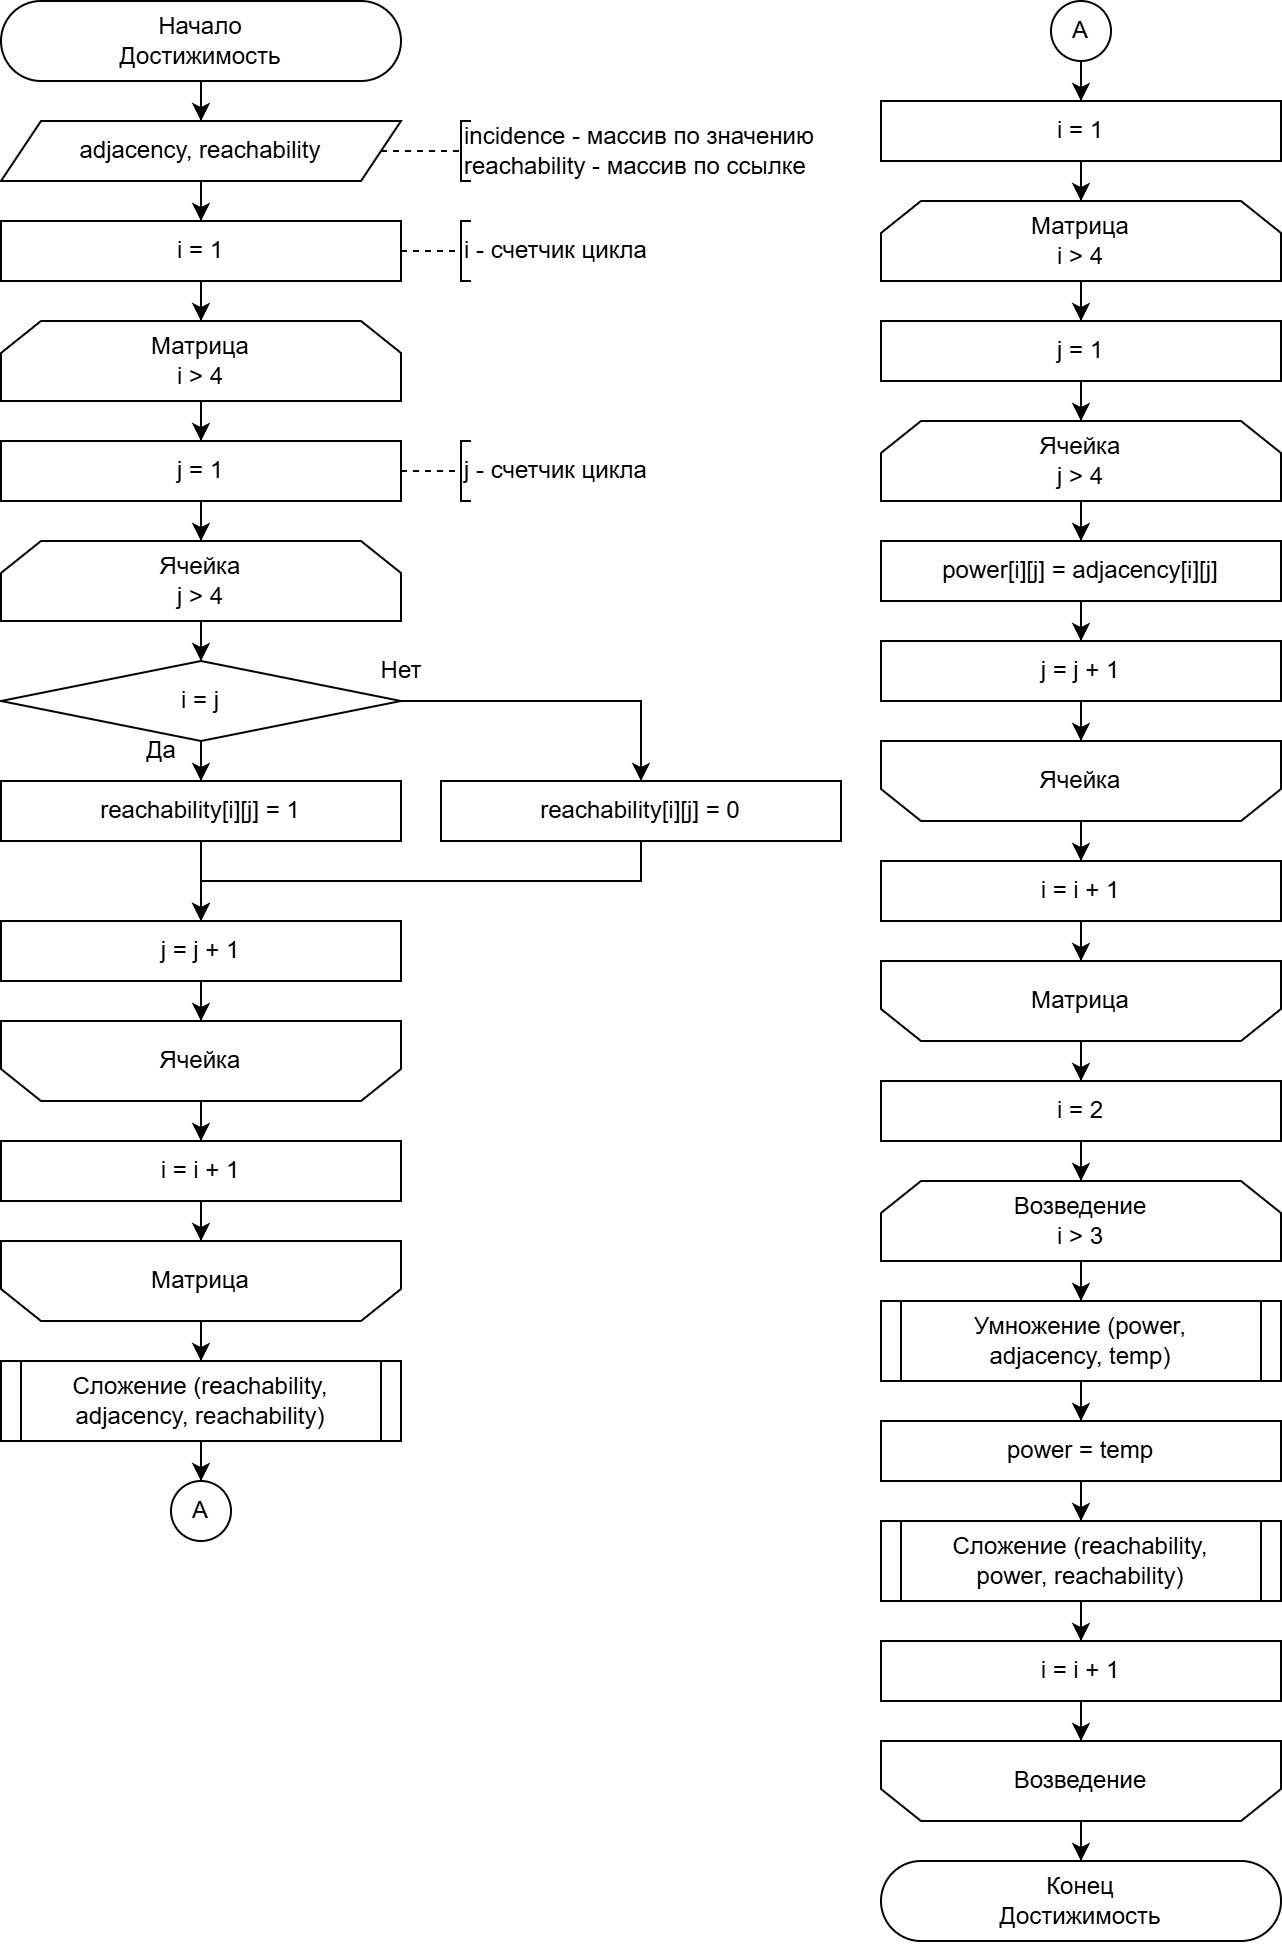
\includegraphics[width=0.7\linewidth]{images/s-4.png}
  \end{figure}
  \begin{center}
    Рисунок 5 – Схема алгоритма формирования матрицы достижимости
  \end{center}

  \pagebreak
  На рисунке 6 представлена схемы подпрограмм транспонирования матрицы, формирования матрицы связности и проверки на связность.

  \begin{figure}[h]
    \centering
    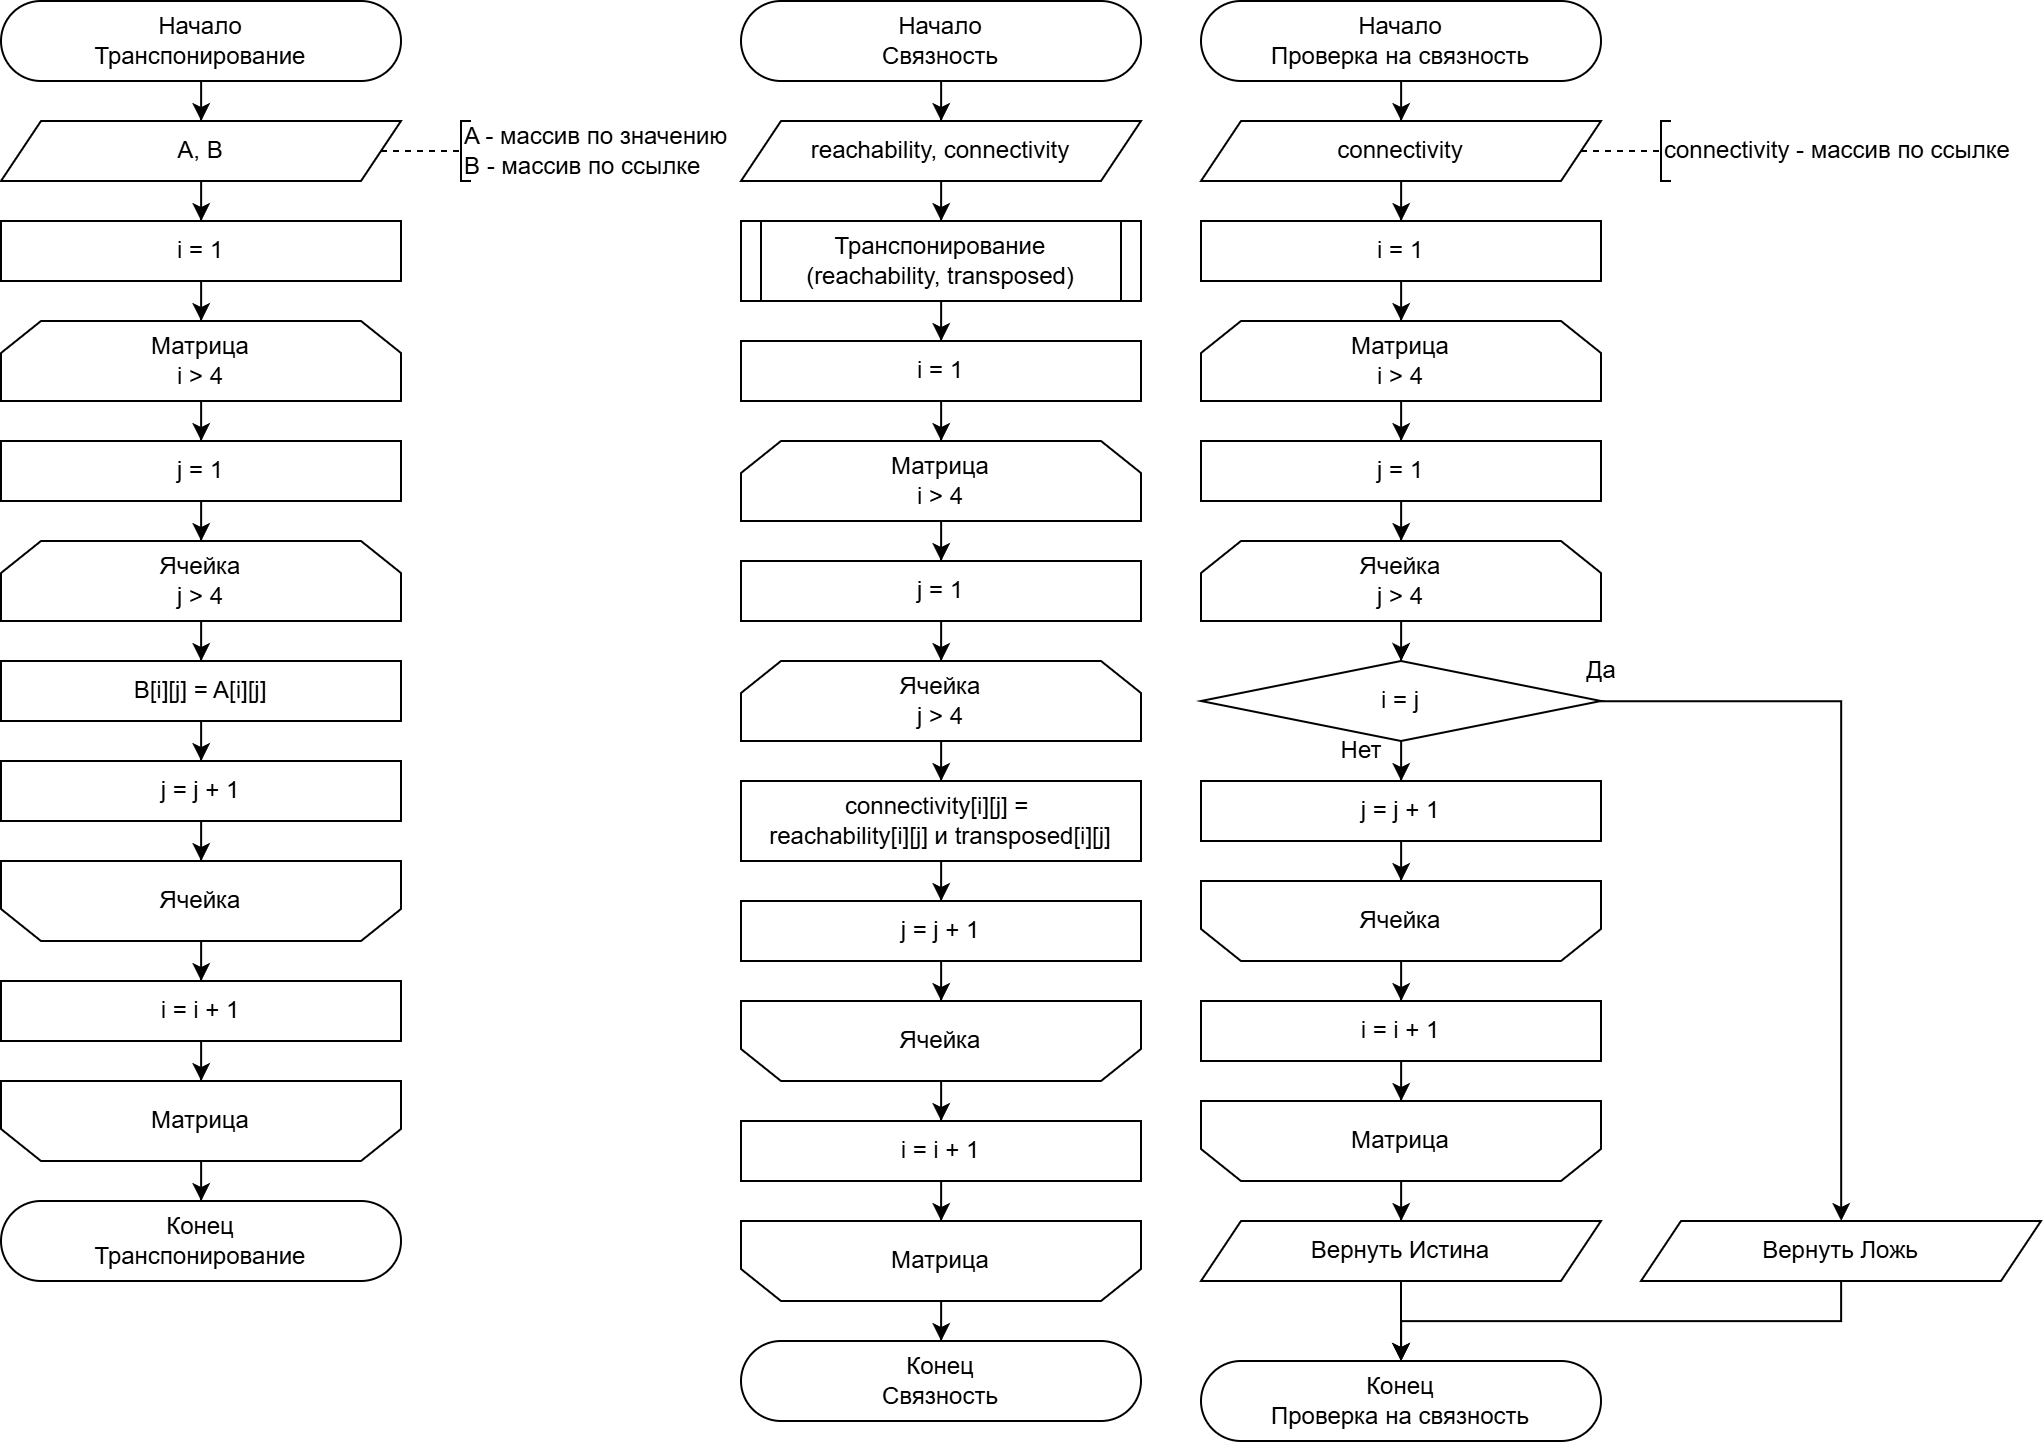
\includegraphics[width=1\linewidth]{images/s-5.png}
  \end{figure}
  \begin{center}
    Рисунок 6 – Схема транспонирования матрицы, формирования матрицы связности, проверки на связность
  \end{center}

  \pagebreak
  На рисунке 7 представлена схема алгоритма основной программы.

  \begin{figure}[h]
    \centering
    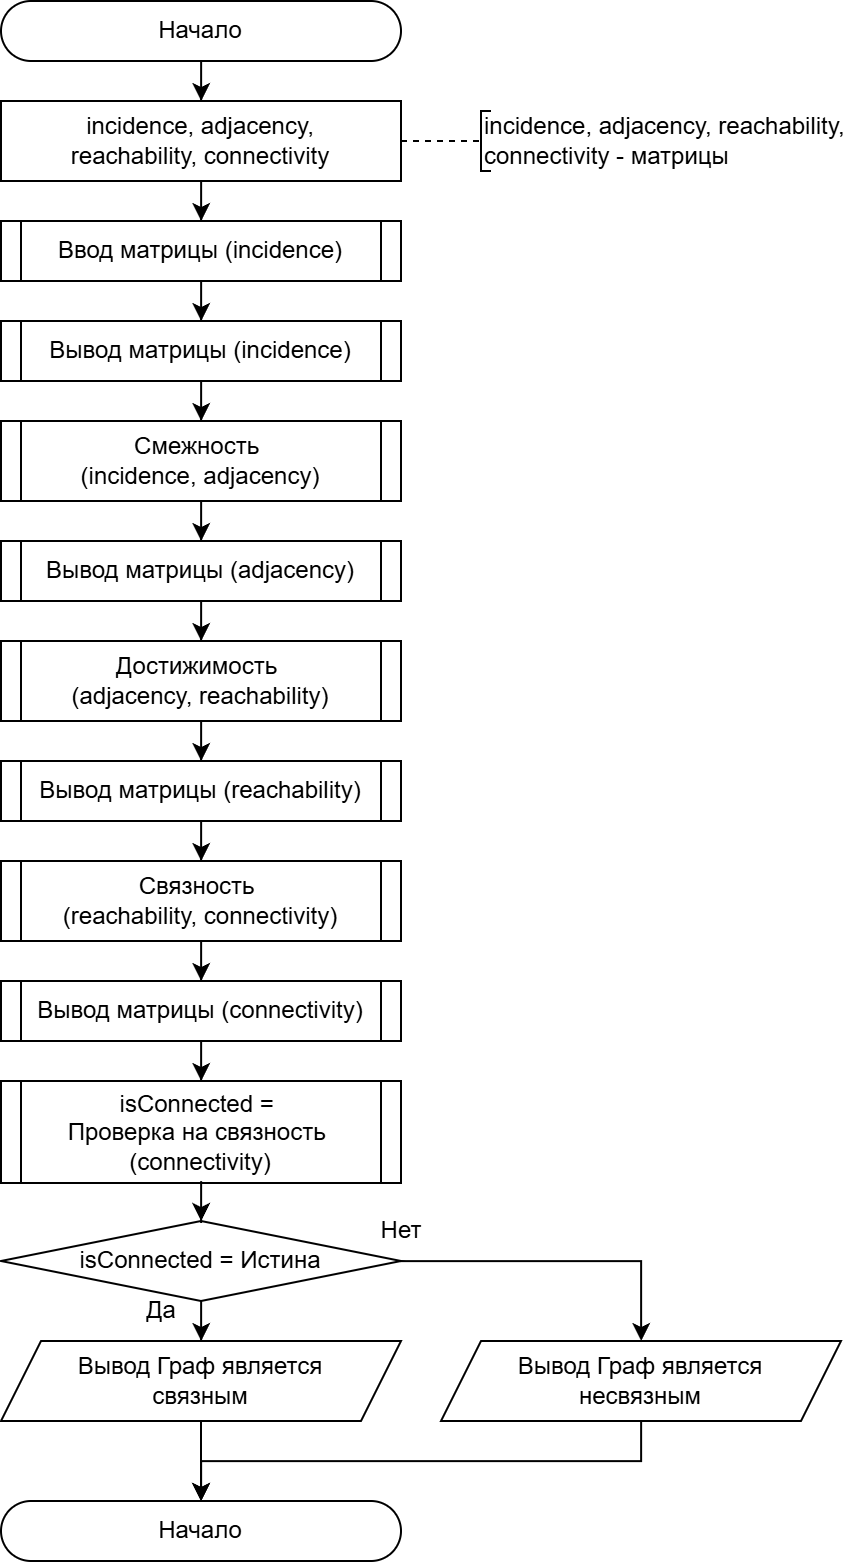
\includegraphics[width=0.63\linewidth]{images/s-6.png}
  \end{figure}
  \begin{center}
    Рисунок 7 – Схема алгоритма основной программы
  \end{center}

  \pagebreak
  При разработке реализована программа, исходный код которой представлен ниже.

  \begingroup
    \linespread{1}

    \begin{Verbatim}[tabsize=2]
{$codepage UTF8}

const
  MAX_SIZE = 4;

type
  TMatrix = array[1..MAX_SIZE, 1..MAX_SIZE] of integer;

procedure PrintMatrix(var matrix: TMatrix);
var
  i, j: integer;
begin
  Write('  ');
  for i := 1 to MAX_SIZE do
    Write(' ', i, ' ');
  Writeln();

  for i := 1 to MAX_SIZE do
  begin
    Write(i, ' ');
    for j := 1 to MAX_SIZE do
      if matrix[i, j] = -1 then
        Write(matrix[i, j], ' ')
      else
        Write(' ', matrix[i, j], ' ');
    Writeln();
  end;
end;

procedure ReadIncidence(var incidence: TMatrix);
var
  fileInput: text;
  fileLine: string;
  i, j, k: integer;
begin
  Assign(fileInput, 'input.txt');
  Reset(fileInput);

  i := 1;
  while not Eof(fileInput) do
  begin
    Readln(fileInput, fileLine);

    j := 1;
    for k := 1 to Length(fileLine) do
      if (fileLine[k] <> ' ') and (fileLine[k] <> '-') then
      begin
        if fileLine[k - 1] = '-' then
          incidence[i, j] := -1
        else if fileLine[k] = '1' then
          incidence[i, j] := 1
        else if fileLine[k] = '2' then
          incidence[i, j] := 2;
        j := j + 1;
      end;
    i := i + 1;
  end;

  Close(fileInput);
end;

procedure ConvertToAdjacency(var incidence, adjacency: TMatrix);
var
  startVertex, endVertex, i, j: integer;
begin
  for j := 1 to MAX_SIZE do
  begin
    startVertex := 0;
    endVertex := 0;

    for i := 1 to MAX_SIZE do
      if incidence[i, j] = 1 then
        startVertex := i
      else if incidence[i, j] = -1 then
        endVertex := i
      else if incidence[i, j] = 2 then
      begin
        startVertex := i;
        endVertex := i;
      end;

    if (startVertex > 0) and (endVertex > 0) then
      adjacency[startVertex, endVertex] := 1;
  end;
end;

procedure MultiplyMatrix(const A, B: TMatrix; var C: TMatrix);
var
  i, j, k: integer;
begin
  for i := 1 to MAX_SIZE do
    for j := 1 to MAX_SIZE do
    begin
      C[i, j] := 0;
      for k := 1 to MAX_SIZE do
        C[i, j] := C[i, j] or (A[i, k] and B[k, j]);
    end;
end;

procedure AddMatrix(const A, B: TMatrix; var C: TMatrix);
var
  i, j: integer;
begin
  for i := 1 to MAX_SIZE do
    for j := 1 to MAX_SIZE do
      C[i, j] := A[i, j] or B[i, j];
end;

procedure ConvertToReachability(const adjacency: TMatrix; 
  var reachability: TMatrix);
var
  temp, power: TMatrix;
  i, j: integer;
begin
  for i := 1 to MAX_SIZE do
    for j := 1 to MAX_SIZE do
      if i = j then reachability[i, j] := 1
      else reachability[i, j] := 0;

  AddMatrix(reachability, adjacency, reachability);

  for i := 1 to MAX_SIZE do
    for j := 1 to MAX_SIZE do
      power[i, j] := adjacency[i, j];
  
  for i := 2 to MAX_SIZE - 1 do
  begin
    MultiplyMatrix(power, adjacency, temp);
    power := temp;
    AddMatrix(reachability, power, reachability);
  end;
end;

procedure TransposeMatrix(const A: TMatrix; var B: TMatrix);
var
  i, j: integer;
begin
  for i := 1 to MAX_SIZE do
    for j := 1 to MAX_SIZE do
      B[j, i] := A[i, j];
end;

procedure ConvertToConnectivity(const reachability: TMatrix; 
  var connectivity: TMatrix);
var
  transposed: TMatrix;
  i, j: integer;
begin
  TransposeMatrix(reachability, transposed);

  for i := 1 to MAX_SIZE do
    for j := 1 to MAX_SIZE do
      connectivity[i, j] := reachability[i, j] and transposed[i, j];
end;

function IsConnected(const connectivity: TMatrix): boolean;
var
  i, j: integer;
begin
  for i := 1 to MAX_SIZE do
    for j := 1 to MAX_SIZE do
      if connectivity[i, j] = 0 then
        Exit(false);
  IsConnected := true;
end;

var
  incidence, adjacency, reachability, connectivity: TMatrix;

begin

  ReadIncidence(incidence);
  Writeln(#10, 'Матрица инцидентности', #10);
  PrintMatrix(incidence);

  ConvertToAdjacency(incidence, adjacency);
  Writeln(#10, 'Матрица смежности', #10);
  PrintMatrix(adjacency);

  ConvertToReachability(adjacency, reachability);
  Writeln(#10, 'Матрица достижимости', #10);
  PrintMatrix(reachability);

  ConvertToConnectivity(reachability, connectivity);
  Writeln(#10, 'Матрица связности', #10);
  PrintMatrix(connectivity);

  if (IsConnected(connectivity)) then
    Writeln(#10, 'Граф является связным')
  else
    Writeln(#10, 'Граф является несвязным');

  Readln;

end.
    \end{Verbatim}
  \endgroup

  \pagebreak
  Экранная форма программы в виде консольного приложения представлена на рисунке 8.

  \begin{figure}[h]
    \centering
    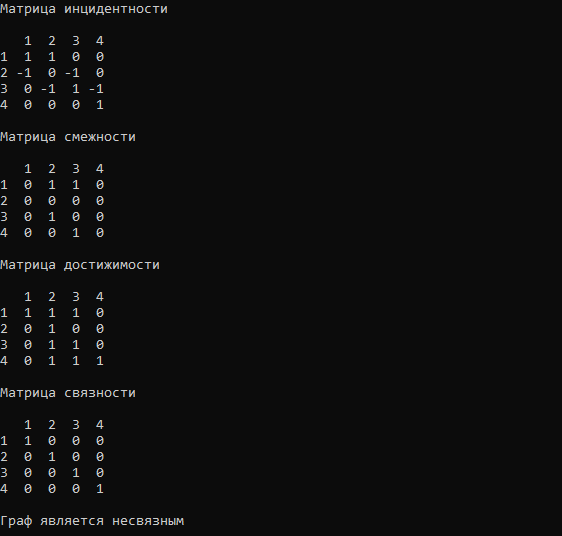
\includegraphics[width=0.9\linewidth]{images/image.png}
  \end{figure}
  \begin{center}
    Рисунок 8 – Консольный интерфейс программы
  \end{center}

  \section*{\hspace{12.5mm}Вывод}
  В процессе выполнения лабораторной работы, при решении предложенных задач, реализована программа на языке Паскаль, которая формирует матрицу связности, определяет является ли граф несвязным.

\end{document}